

\chapter{Introduction}
\label{sec:ch1}

\section{Concurrent Software Correctness}

In the life-cycle of computer programs, software testing and debugging play essential roles.
%
Many approaches have been developed to test and debug software at different layers and from various aspects.
%
Traditional and basic debugging techniques such as ``printf'' debugging, interactive debugging \cite{ddt, totalview}, memory dumps, and profiling have been used widely in software development.
%
%
However, modern concurrent system architectures and programming languages require novel software debugging techniques~\cite{hpcdoe}.
%
With the high growth in computation power and modern languages, programs are getting more sophisticated, complex, large, and heterogeneous to exploit the processing power efficiently (e.g., distributed memory and shared memory systems in  Cloud and High-Performance Computing - HPC).
%
Locating bugs in such programs is notoriously challenging because 1)~the interleaving space grows exponentially with the number of processing units, 2) concurrent bugs are difficult to reproduce due to the non-deterministic nature of concurrent software, and 3) root-causing misbehaved executions of a concurrent program are non-trivial due to the complex interactions between concurrent program components.
%
Researchers have developed techniques and tools to detect, prevent, and fix concurrent bugs in different levels of abstraction from multiple perspectives.
%
Depending on the characteristics of target bugs \cite{shanlu-mistakes-asplos08}, there are some advantages and limitations to each approach.
%
Static analyzers (\ie, methods that analyze software without actually executing the program) offer rigorous guarantees, but they are often not practical for large-scale real-world programs.
%
While dynamic analyzers (\ie, methods that analyze software based on execution evidence) cover a broader class of programs, they incur overhead to the program execution and may miss uncommon bugs.
%
Hybrid analyzers (\eg, testing coverage analysis) combine ideas from both techniques to deliver reliable and practical debuggers.
%
This dissertation has combined ideas from the broad spectrum of concurrency debugging approaches and implemented several frameworks and toolchains to assist parallel software developers in locating flaws in the program by automated and efficient data collection and analysis.

\subsection{Background}
Debugging concurrent programs require insight into the behavior of target bugs.
%
A bug's behavior is described by its /textit[cause] and its \textit{symptom} during execution.
%
Adopting form the taxanomy proposed for concurrent Go bugs~\cite{tu-concurrentBugs-asplos19}, we generally categorize common concurrency bugs in both shared and distrubutted memory systems based on the \textit{symptom of the bug} (figure \ref{fig:ch1_concBugs}).
%
This work aims not to focus on a specific bug class but rather to provide general tools to analyze the symptoms of unexpected behaviors in HPC and Cloud systems (i.e., shared memory and distributed memory systems) to help locate their cause.

\subsubsection{Blocking Bugs}
Blocking bugs lead the execution of the program into a \textit{halt} state and prevent the program from making progress and reaching its final state.

\begin{itemize}
  \item \textbf{Deadlock} is a situation where one or more processes in a system cannot proceed because they are blocked waiting for a shared resource held by another process. More generally, deadlock occurs when a process is waiting for an external \textit{signal} from another process which is also attempting to acquire a resource held by other processes.
  \item \textbf{Livelock} is a condition where a thread is waiting for a resource that will never become available. It is similar to deadlock except that the state of the process involved in the livelock constantly changes regarding each other, non progressing.
  \item  \textbf{Starvation} occurs in systems with different priorities for the execution of processes when one or more processes are constantly delayed indefinitely due to the higher priority processes receiving the required resources.
\end{itemize}


\subsubsection{Non-Blocking Bugs}
Non-blocking bugs cause the program to produce incorrect results. The program execution terminates, but the generated output is invalidated because of the lack of proper \textit{serilaization} for concurrent memory accesses.
\begin{itemize}
  \item \textbf{Order violation} is the violation of the expected order of at least two memory accesses which produce corrupted results.
  \item \textbf{Atomicity violation} refers to the situation when two blocks of code (\ie, finite sequences of statements) execute concurrently and produce inconsistent results depending on the non-deterministic order of executions.
  \item \textbf{Data race} occurs when at least two concurrent threads access the same memory location, and at least one of the accesses is \textit{write}.
\end{itemize}

\begin{figure}[t]
\centering
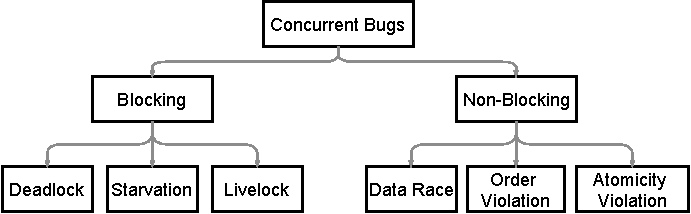
\includegraphics[width=.9\textwidth]{dissertation_intro_bugs.pdf}
\caption{Taxanomy of concurrent bugs}
\label{fig:ch1_concBugs}
\end{figure}

\subsubsection{Concurrent Debugging}
Figure \ref{fig:ch1_concDebugging} displays the general taxonomy of methods for tackling concurrency debugging challenges.
%
\textbf{Testing} exercises the program behavior over a set of inputs (manually written tests) or over the schedule space (feasible interleavings) to detect errors. Although testing effectively reveals flaws of the program, it does not guarantee the program's bug freedom.
\textbf{Model checking} exhaustively test the program to cover possible control flow paths and verify the program properties. However, due to scalability problems, model checking is typically done symbolically and up to a certain bound; thus, they rarely achieve a guarantee.
\textbf{Tracing} collects evidence from program execution, enabling offline analysis of the program's dynamic behavior. Similar to tracing, \textbf{Record and Replay} technique captures a single execution of the target program for later replay and analysis of the program's non-deterministic behavior. Both methods usually incur overhead to the native execution of the program and require sophisticated mechanisms to make them practical for real-world programs and large-scale executions. \textbf{Theorem Proving} techniques, in principle, prove a system to be free of flaws often through verifying type systems. The enormous effort needed to use these tools makes them most appropriate for new implementations of small, critical cores. \textbf{Visualization} techniques provide transparent representations of complex concurrent execution of the program for developers to analyze visually.

In this dissertation, we combine and apply methods from \textit{tracing} (chapters \ref{sec:ch2} and \ref{sec:ch4}), \textit{record and replay} (chapters \ref{sec:ch2},\ref{sec:ch3} and \ref{sec:ch4}), \textit{testing} (chapter \ref{sec:ch4}), and \textit{visualization} (chapters \ref{sec:ch3} and \ref{sec:ch4}) to facilitate the process of concurrent debugging.
\begin{figure}[t]
\centering
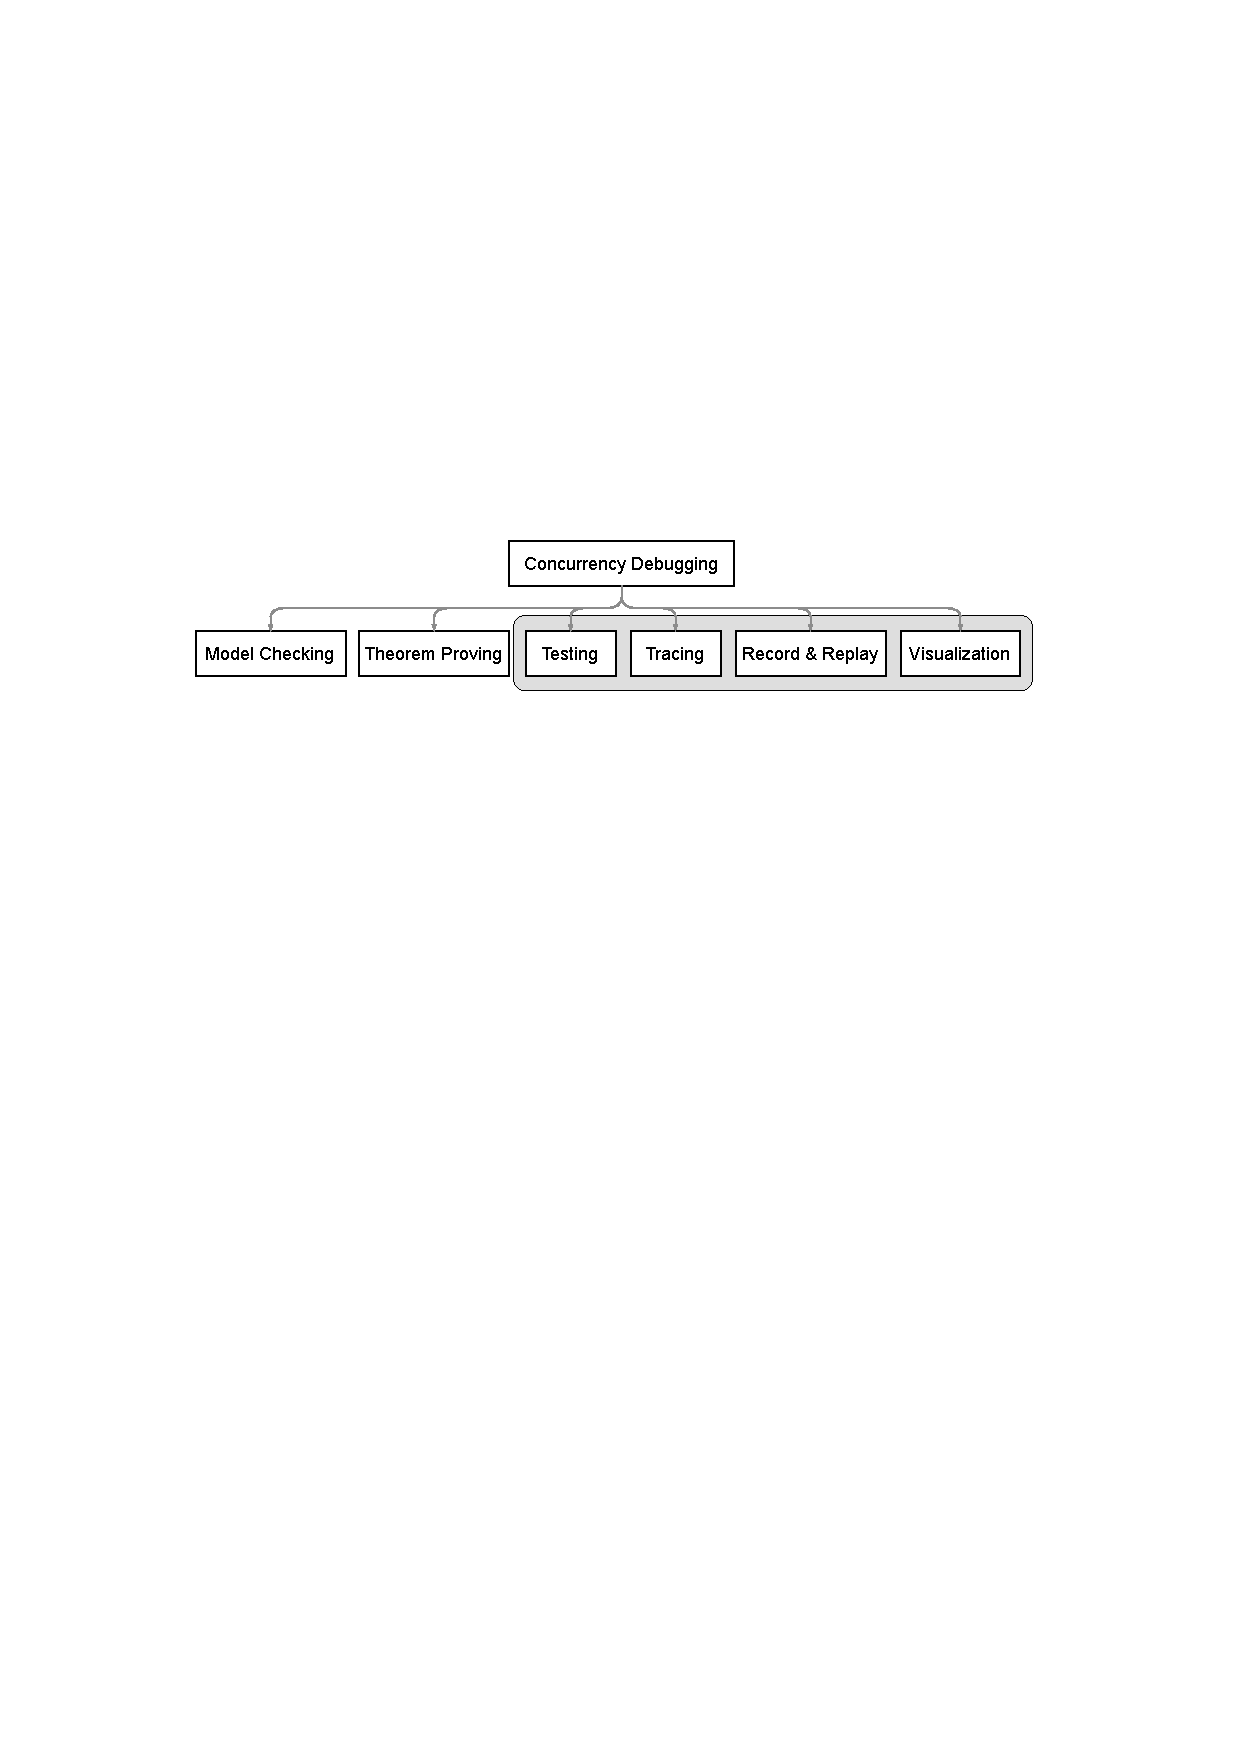
\includegraphics[width=1\textwidth]{dissertation_intro_approaches2.pdf}
\caption{Taxanomy of concurrent debugging approaches. The highlighted area shows the techniques that we employed in this disseration.}
\label{fig:ch1_concDebugging}
\end{figure}



\section{Dissertation Statement}

This dissertation aims to facilitate the concurrent debugging process by providing efficient data collection and effective information retrieval mechanisms to target real-world software and bugs.
%
With that being said, our thesis statement is the following:

\begin{quote}
Efficiently collecting data and systematically analyzing them is essential to gaining insight into the behavior of complex programs and help developers fix the flaws of the program. Also, given the rich set of concurrency primitives in modern languages, one needs to articulate nuanced concurrency coverage metrics and demonstrate their attainment.
\end{quote}

\section{Contributions of the Dissertation}
In this dissertation, we present different contributions to facilitate concurrent debugging using efficient tools and automated frameworks.
%

First, we introduce \parlot (Chapter \ref{sec:ch2}), a new tracing approach that makes it possible to capture the whole-program call-return, call-stack, call-graph, and call-frequency information, including all library calls, for every thread and process of HPC applications at low overhead in both space and time.
%
\parlot is equipped with a new incremental data compression algorithm to drastically reduce the required tracing bandwidth (average of 56 kB/s per core), thus enabling the collection of whole-program traces, which would be infeasible without on-the-fly compression.
%
\parlot can instrument x86 applications at the binary level (regardless of the source language used) to collect whole-program call traces with the compression ratio of up to 21,000.

Second, we present DiffTrace (Chapter \ref{sec:ch3}), a series of automated data abstraction, representation, and visualization techniques that differentiate the collected \parlot traces and narrows the search space down to just a few candidates of buggy traces.
%
In DiffTrace, we employ {\em concept lattices} to amalgamate the collected traces and hierarchically cluster them based on features extracted from the structure of traces.
%
DiffTrace also utilizes the rigorous notion of Nested Loop Representations (NLRs) for summarizing traces and representing loops in a manner that informs the developer engaged in debugging.
%
We evaluate the effectivness of DiffTrace by locating artificial bugs injected to ILCS \cite{ilcs}, a hybrid (MPI + OpenMP) HPC framework.

Third, we illustrate \goat (Chapter \ref{sec:ch4}), a testing and analysis framework for concurrent Go applications that provides for whole-program trace collection (via an enhancement to the standard tracer package) and knowledge discovery about the program's dynamic behavior.
%
We show the effectiveness of controlled preemptions for concurrency bug exposure in the context of a real-world language.
%
We demonstrate the effectivness of \goat by detecting all 68 GoKer \cite{yuan-gobench-cgo21} blocking bugs, many of which are undetected by existing tools.
%
Lastly, we propose a set of coverage requirements to measure testing quality in CSP-like concurrent languages.
The proposed metrics characterize the dynamic behavior of concurrency primitives, enabling measurement of quality and progress of schedule-space exploration.


\section{Organization of the Dissertation}
This dissertation is organized as follows: In Chapter \ref{sec:ch2}, we present the design and evaluation of \parlot, the whole-program tracing mechanism; Chapter \ref{sec:ch3} illustrates the series of trace abstractions and representations towards locating the flaw by clustering and diffing traces; with Chapter \ref{sec:ch4}, we describe the end-to-end analysis and testing framework for concurrent Go applications called \goat, and propose a set of concurrency coverage metrics to measure the quality of schedule space exploration; finally, in Chapter \ref{sec:ch5}, we summarize all the contributions and conclude the dissertation.
